\documentclass[10.5pt]{config}

\major{生物医学工程}
\name{卢星余}
\partner{} % 签名栏
% \title{}
\stuid{3220100425}
\date{2025年2月27日}
\lab{教6-204}
\course{生物医学图像处理}
\instructor{吴丹}
\grades{}
\expname{lab1} % 实验名字
\exptype{} % 实验类型

\begin{document}

% \maketitlepage % 封面
% \maketoc % 目录
\makeheader % 首页头部


\section{实验目的和要求}
使用python,对图像处理的基本操作获得初步的认识;了解灰度图和彩色图在python中的表现方式;尝试使用
pyhton中matplotlib包中相关函数对图像进行简单的操作。
\section{实验内容和原理}
\subsection{Project1 创建图像}
\begin{itemize}
    \item 创建一个 $256 \times 256$ 大小的有一个圆环在中心的灰度图像
    \item 创建两个顶点为 $0$ 并在对角线上线性增加到 $255$ 的灰色图像
\end{itemize}
\subsection{Project2 灰度级别调整}
\begin{itemize}
    \item 读取 lab1.npy 或 lab1.mat 文件
    \item 编写程序将灰度级别降低至 $2^n$ 级,定义函数 $y = f(x, n)$,其中 $n$ 为函数的输入参数
    \item 显示具有 256 级(n=8)、64 级(n=6)和 16 级(n=4)的调整后图像
\end{itemize}
\subsection{Project3:图像缩放与细节分析}
\begin{itemize}
    \item 沿图像绘制一条直线,对比分析以下三种情况的细节表现:
    \begin{itemize}
        \item 原始图像
        \item 将图像尺寸缩小至 $1/N$
        \item 将缩小后的图像尺寸放大至原尺寸的 $N$ 倍
    \end{itemize}
\end{itemize}
\subsection{Project4:颜色叠加分析}
\begin{itemize}
    \item 生成二值掩膜:通过图像强度 $I > T$ 进行阈值分割(其中 $T$ 为预设阈值)
    \item 生成颜色叠加图像:将掩膜叠加至红色通道(RGB格式下保留原图其他通道,仅红色通道应用掩膜)
\end{itemize}
\section{实验设备及材料}
Python
\clearpage
\section{实验方法和步骤}
根据实验要求撰Python脚本运行
\section{实验结果与分析}
\subsection{Project1 创建图像}
\begin{figure}[!htbp]
    \centering
    \begin{minipage}[b]{0.45\linewidth}
        \centering
        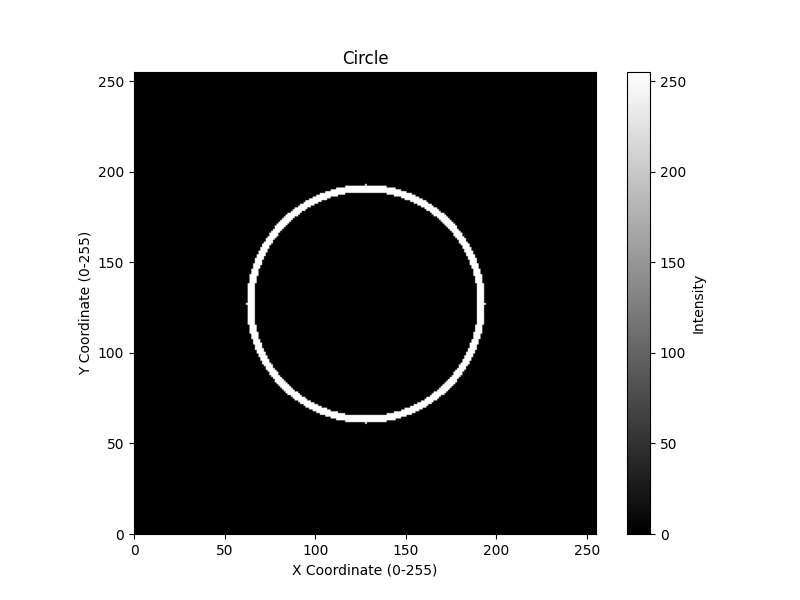
\includegraphics[width=1.0\textwidth]{figures/circle.png}
        \caption{circle.png}
    \end{minipage}%
    \begin{minipage}[b]{0.45\linewidth}
        \centering
        
\includegraphics[width=1.0\textwidth]{figures/diagonal_gradient.png}
        \caption{diagonal\_gradient.png}
    \end{minipage}
\end{figure}
\subsection{Project2 灰度级别调整}
\begin{figure}[htbp]
    \centering
    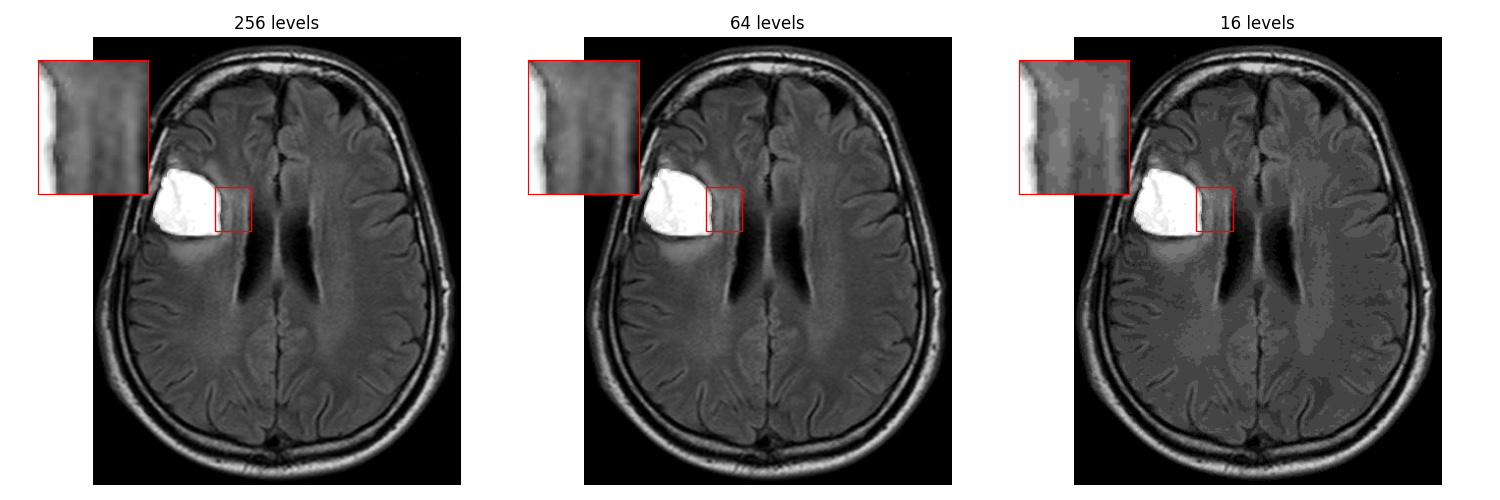
\includegraphics[width=1.0\linewidth]{figures/intensity_levels.png} % 数字表示放缩比例
    \caption{intensity\_levels.png} % 图片标题
    \label{fig:intensity_levels} % 图片tag,用于交叉引用
\end{figure}
我们可以发现16级的灰度明显比256级和64级的更模糊,而256级和64级的区别不大
\clearpage
\subsection{Project3:图像缩放与细节分析}
\begin{figure}[htbp]
    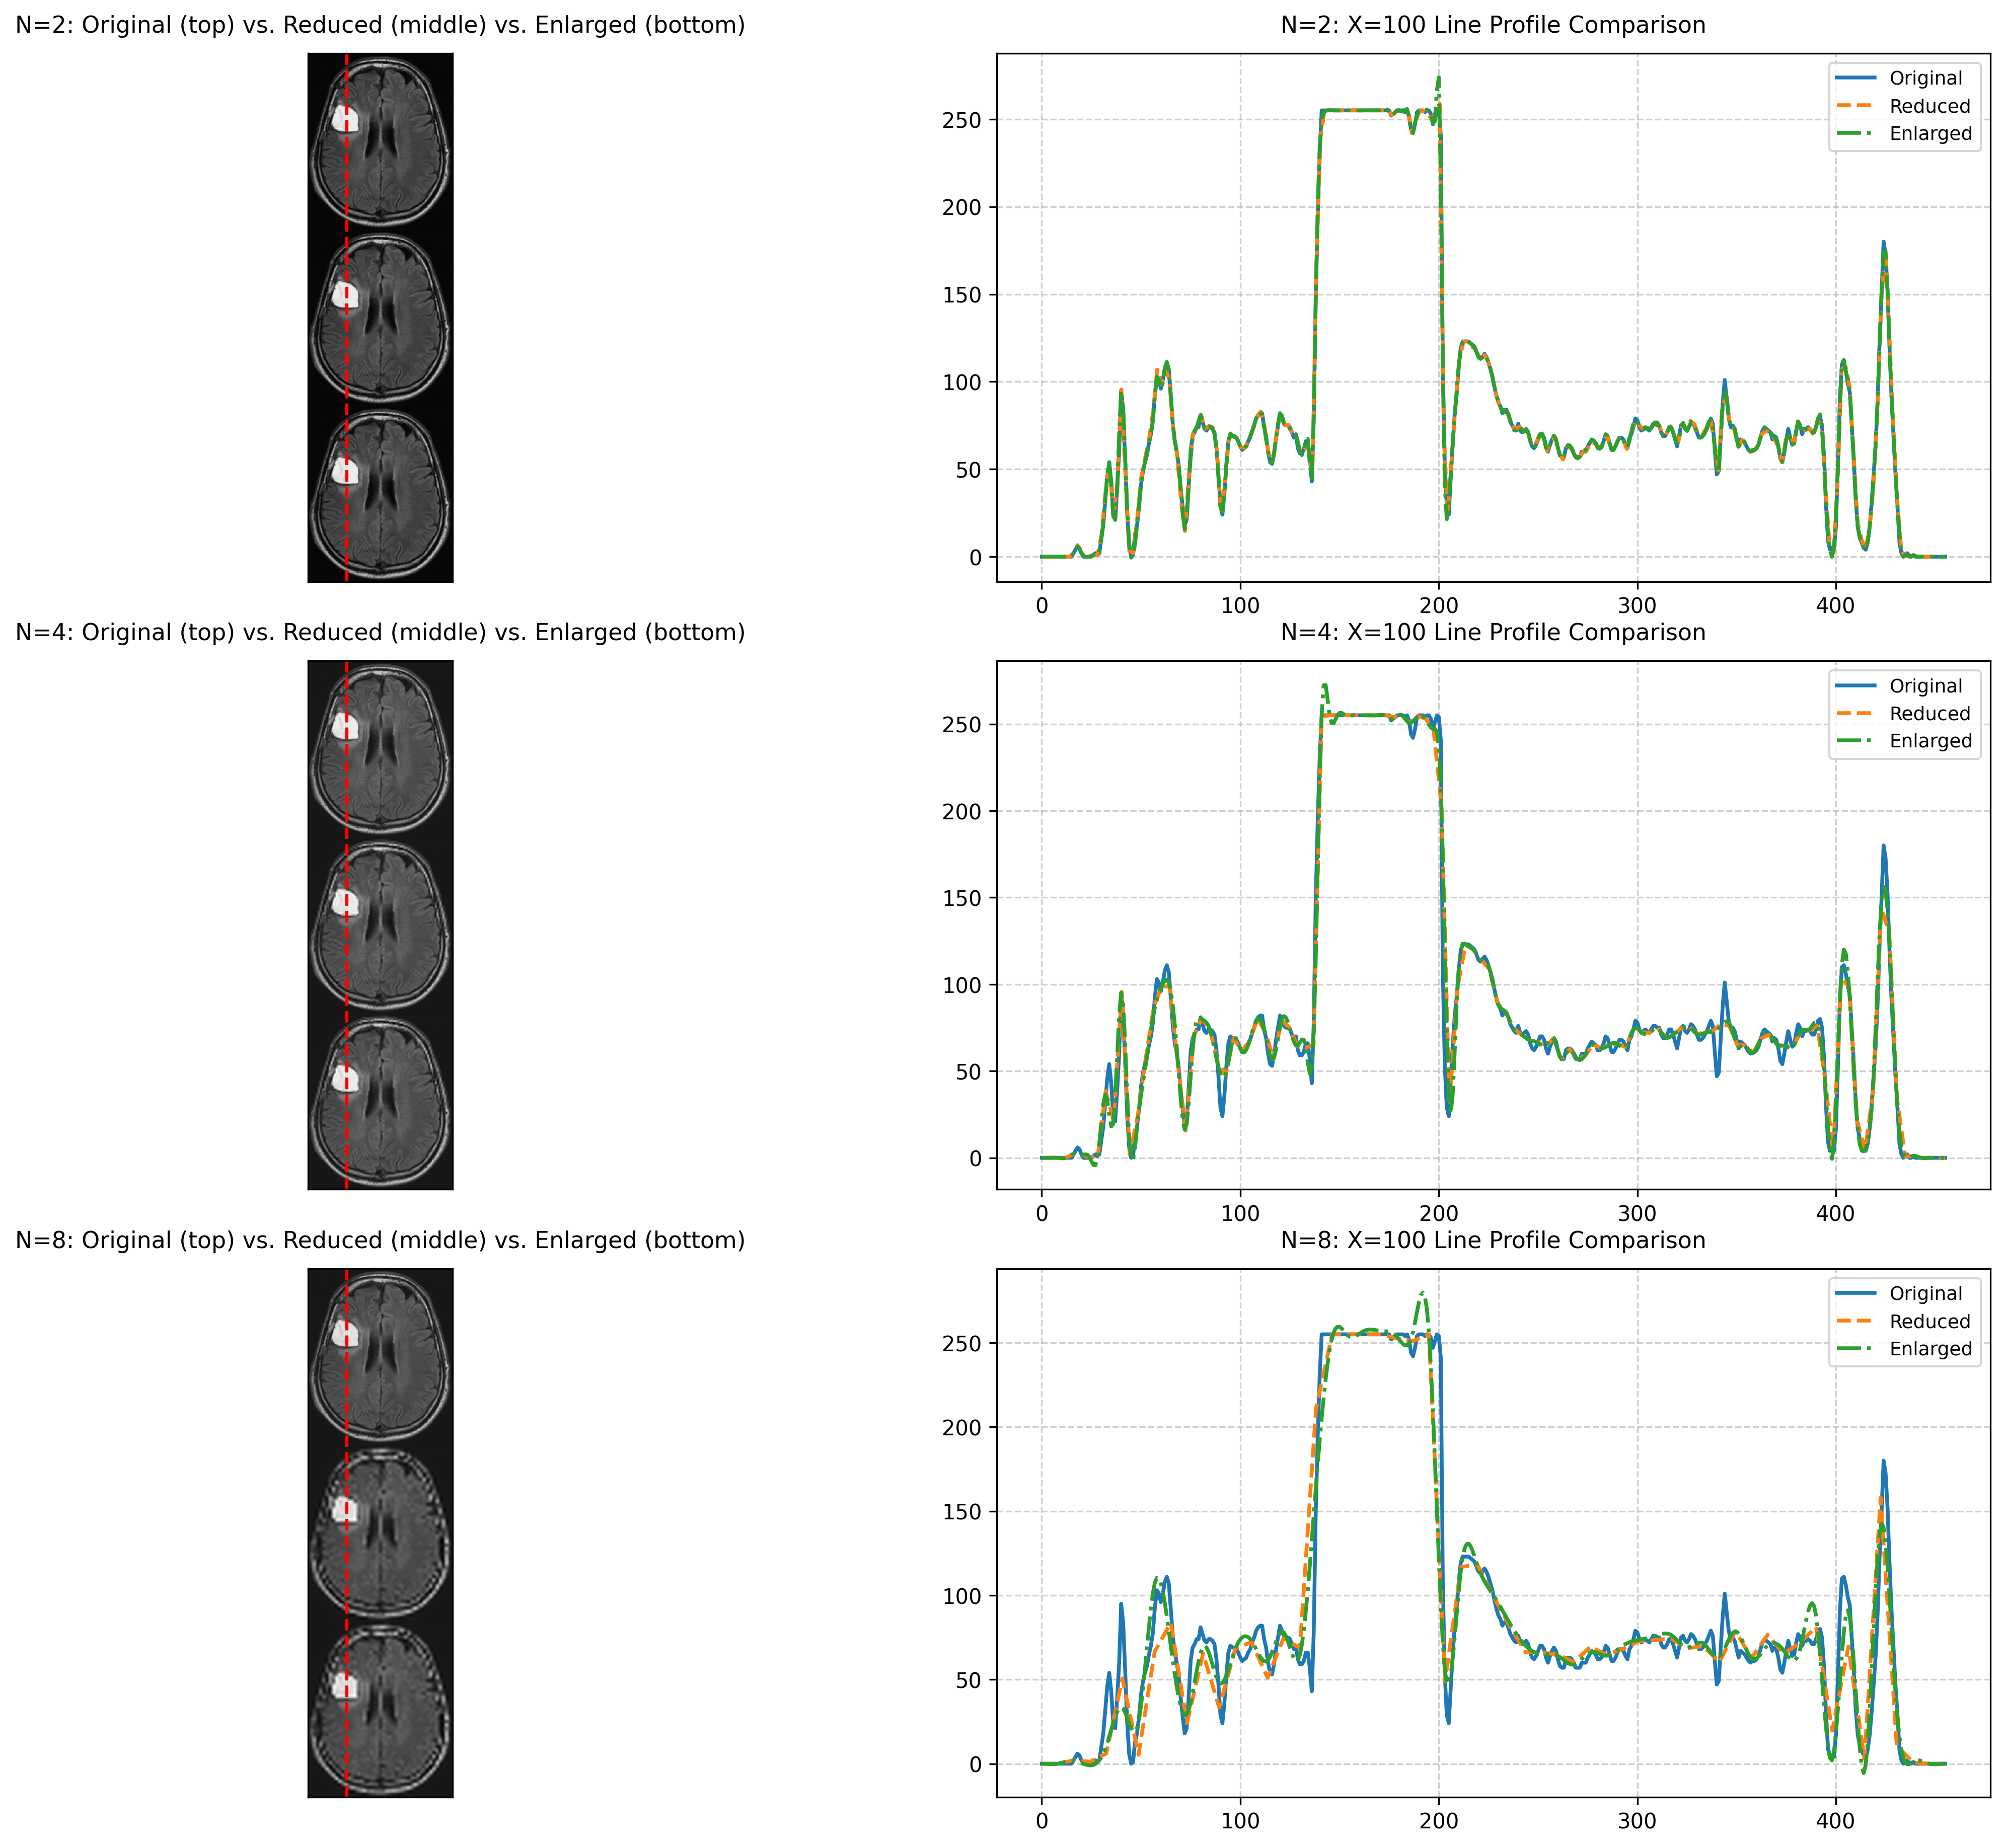
\includegraphics[width=1.0\linewidth]{figures/scaling_comparison_multiple.png} % 数字表示放缩比例
    \caption{scaling\_comparison\_multiple.png} % 图片标题
    \label{fig:scaling_comparison_multiple} % 图片tag,用于交叉引用
\end{figure}
我们可以发现N=2和N=4的缩放造成的细节损失不是很明显,但是N=8的缩放造成的细节损失在肉眼观测和图像都非常明显
\clearpage
\subsection{Project4:颜色叠加分析}
\begin{figure}[htbp]
    \centering
    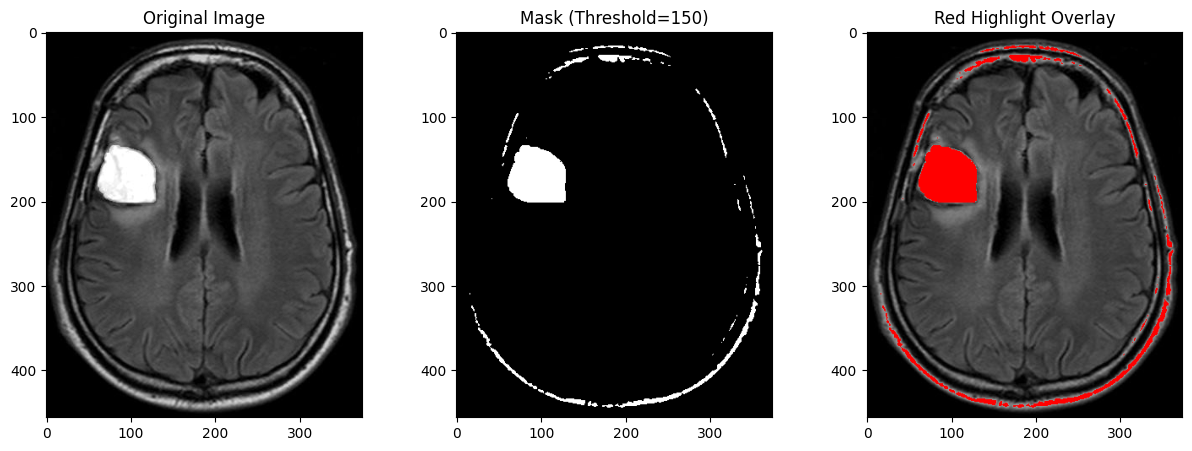
\includegraphics[width=1.0\linewidth]{figures/color_overlay_150.png} % 数字表示放缩比例
    \caption{color\_overlay\_150.png} % 图片标题
    \label{fig:color_overlay_150} % 图片tag,用于交叉引用
\end{figure}
\begin{figure}[htbp]
    \centering
    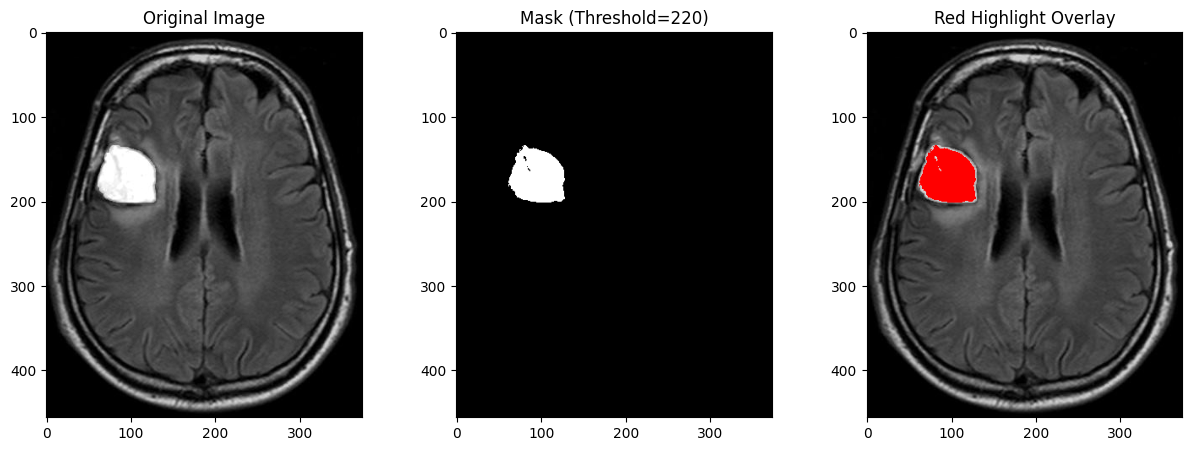
\includegraphics[width=1.0\linewidth]{figures/color_overlay_220.png} % 数字表示放缩比例
    \caption{color\_overlay\_220.png} % 图片标题
    \label{fig:color_overlay_220} % 图片tag,用于交叉引用
\end{figure}
通过阈值判断设置掩膜应该可以用于分割MRI成像中的不同组织(脑脊液,灰质等)

总体来看完成了实验要求内容,实验结果符合理论情况
\section{讨论、心得}
通过本次实验,初步了解了数字图像的矩阵表述方式和实际处理方式,包括图像的创建、放大、缩小、灰度等级转化;对三
通道的彩色图有了了解,包括灰度图与彩色图的转化、设置阈值、设置掩膜和覆盖图等操作。突然发现灰度值的实际上在某种意义上是离散表示(像素也是),从这个角度重新理解Vision Transformer对图像处理的离散token化似乎更好理解一点(传统的VIS切patch是在二维的整体图像上,能不能试试在纵向的灰度上也切patch,:l我瞎猜的)
\end{document}